\section{Ergebnisse}


\subsection{Implementierung des Frontends}

\begin{itemize}
	\item Tools
	\begin{itemize}
	
		\item TypeScript
		\begin{itemize}
			\item Typ-Sichere version von JavaScript
			\item Compiliert auf JavaScript
		\end{itemize}
		
		\item npm
		\begin{itemize}
			\item Three.js als dependency
			\item AR.js von github
			\begin{itemize}
				\item TypeScript declaration file
			\end{itemize}
		\end{itemize}
		
		\item webpack
	\end{itemize}
	
	\item Workflow + Klassen + Funktionen + Sequenz-Diagramm
	
	\item GUI
	\begin{itemize}
		\item Spannt eine GUI ebene auf mit der sich eine ebene zum Filtern der Vektor daten aktivieren und einstellen lässt
		\item Triggert gewisse Events, bei Änderungen
		\begin{itemize}
			\item Wird genutzt um Filer an zu passen
		\end{itemize}
		\item Daten werden bei anfrage an Backend genutzt
	\end{itemize}
\end{itemize}



\subsection{Implementierung des Backends}

\begin{figure}
	\centering
	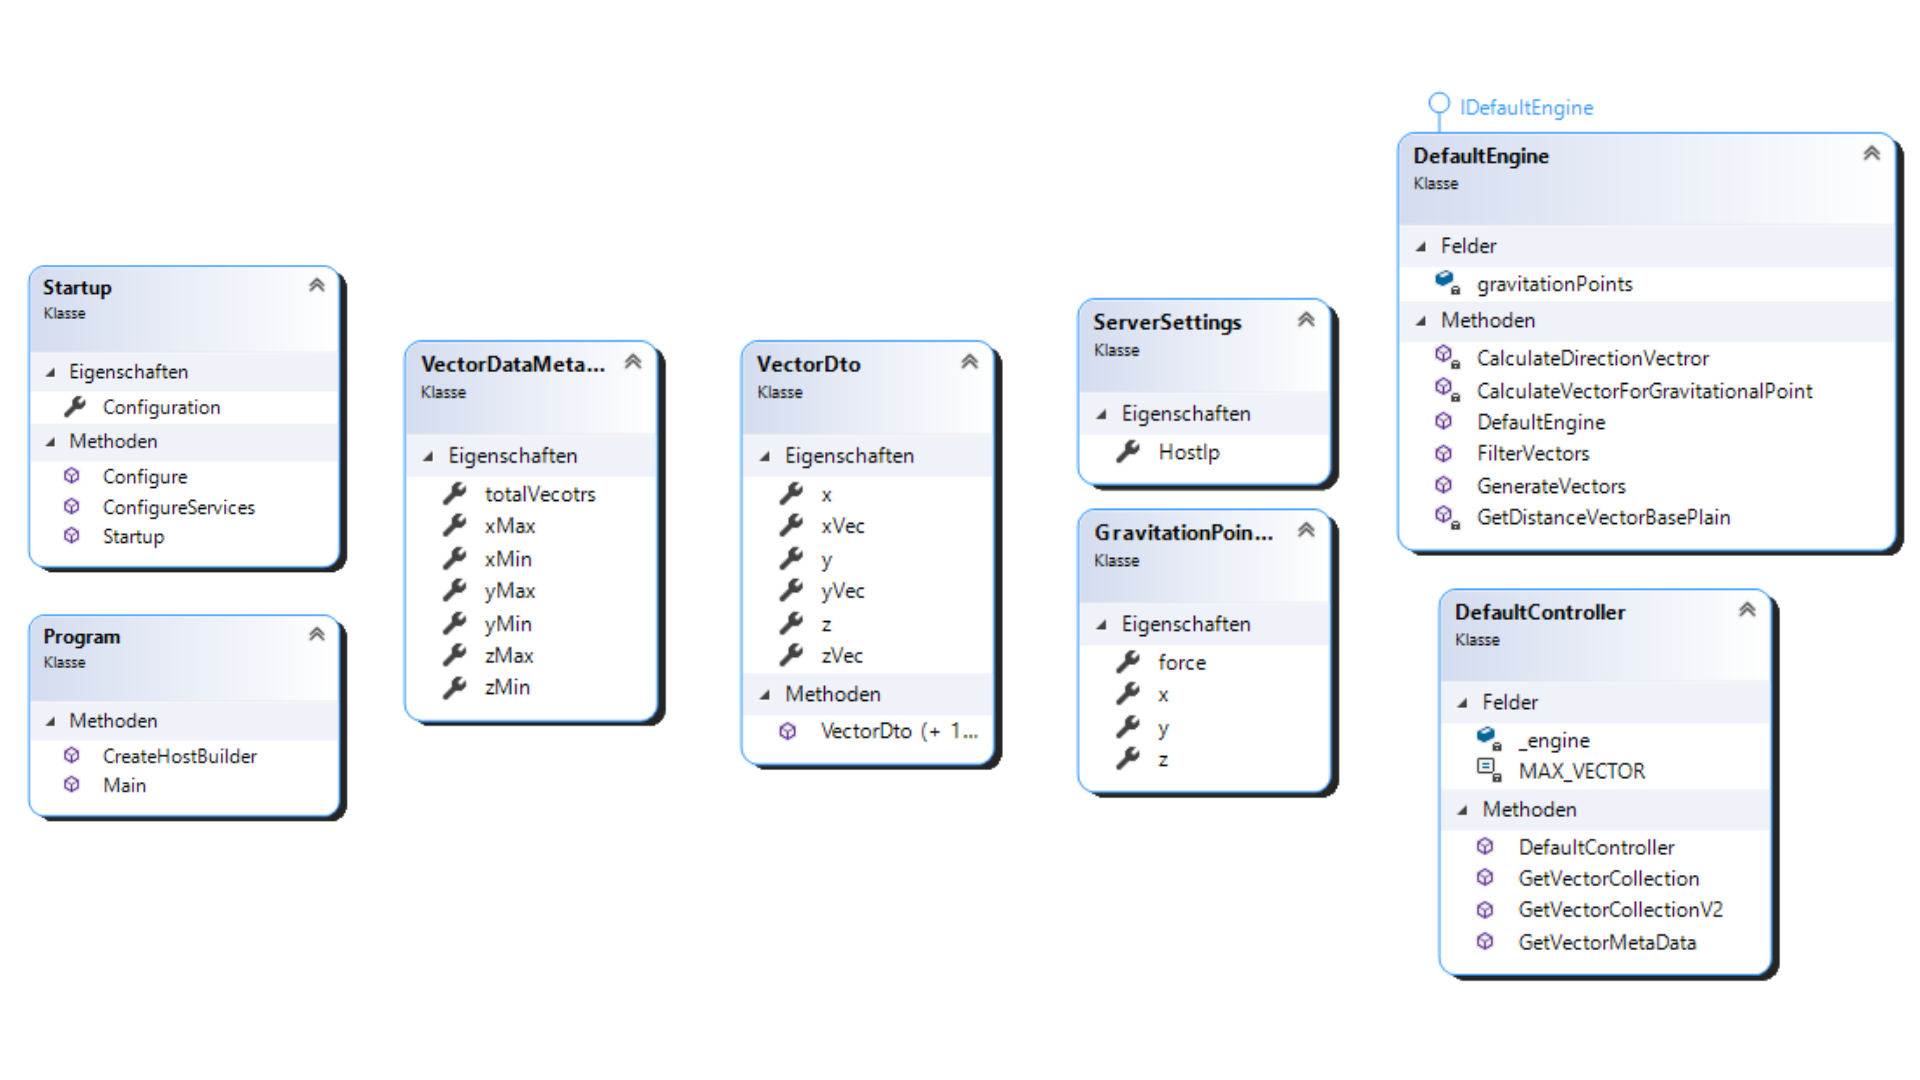
\includegraphics[width=\linewidth]{images/backend/classDiagram}
	\caption{System Klassen, Dto Klassen und Controller und Engine Klassen}
	\label{fig:ClassDiagram}
\end{figure}

Die Backend API wird in Asp.NetCore (C\#) implementiert. Das Framework wurde gewählt, da es kostenlos und opensource ist und da es sowohl auf Linux als auch auf Windows lauffähig ist (vgl. DotNet Download page \cite{DotNetDownloadPage}). Außerdem liefert NetCore mit ASP nativ eine IIS Webapplikation Funktionalität mit, sodass die API schnell und einfach umzusetzen ist, ohne einen großen web hosting overhead zu erzeugen. Grundsätzlich besteht das Programm aus drei Klassen Gruppen, den System Klassen, den Controller und Engine Klassen und den data transfer object (Dto) Klassen (siehe Abbildung \ref{fig:ClassDiagram}).\\
Die Klasse Programm besitzt vordefinierten code zur Instanziierung des WebHosts.

\begin{codefig}
	\centering
	\lstset{style=sharpc}
	\begin{lstlisting}
 public static void Main(string[] args)
        {
            var config = new ConfigurationBuilder()
                .AddJsonFile("appsettings.json", optional: false)
                .Build();
            var serSet = new ServerSettings();

            config.GetSection("ServerSettings").Bind(serSet);

            CreateHostBuilder(args, serSet).Build().Run();
        }

        public static IHostBuilder CreateHostBuilder(string[] args, ServerSettings serverSettings) =>
            Host.CreateDefaultBuilder(args)
                .ConfigureWebHostDefaults(webBuilder =>
                {
                    webBuilder.UseStartup<Startup>();
                    webBuilder.UseUrls(serverSettings.HostIp);
                });
	\end{lstlisting}
	\caption{Methoden der Program Klasse}
	\label{codefig:Program.cs}
\end{codefig}

\begin{itemize}
	\item Framework: Netcore (C\#)
	\begin{itemize}
		\item Ausgewählt da
		\item NetCore sowohl auf Linux alsauch Windows verfügbar
		\item ASP Netcore eine stabile und aktuelle grundlage für WebApplications und WebAPIs bietet (liefert viele funktionen nativ mit)
	\end{itemize}
	
	\item Klassendiagramm
	\begin{itemize}
		\item Einzelne Klassen beschreiben
	\end{itemize}
		
	\item CORS
	\begin{itemize}
		\item Implementierung:
		\begin{itemize}
			\item Hinzufügen einer Policy in Netcore, welche alle Origins erlaubt
		\end{itemize}
	\end{itemize}
	
	\item Implementierung der Endpunkte
	\begin{itemize}
		\item Daten auslieferung/gewinnung
		\begin{itemize}
			\item Simulation der daten früher via Gravitationsmodell
			\item Simulation jetzt durch ausliefern vorberechneter und vorgegebener Simulationsdaten
		\end{itemize}
				
		\item Filterung
		\item Meta Info auslieferung
	\end{itemize}
		
	\item Ausliefern der statischen daten und aufbereitung mit DirecotryBrowser durch NetCore mitgelieferten funktionen
	\begin{itemize}	
		\item Hinzufügen eines FileExtensionContentTypeProvider für nicht nativ unterstützte Dateien (.dat, .patt, .mtl, .obj)
	\end{itemize}
		
	\item Hosten in Azure zu entwicklungszwecken
\end{itemize}


